\section{Solving a toy example}
Using this, we are now in a position to solve simple partial differential
equations. For benchmarking purposes, consider:

\begin{eqnarray*}
\frac{dy}{dx} & = & \frac{1}{x}
\end{eqnarray*}

The solution to this equation is: $y=\log\left(x\right)+c$. Solving
this using the gradient backpropagation, we get the remarkable graph {\autoref{fig:log}}

An implementation of this method (in C++) is available at:
[{\url{https://github.com/aravindhv10/CPP_Wrappers/tree/master/LatestHeaders}}].
The implementation so far only works on the CPU (uses CPU blas and doesnot run on GPU), this result was obtained with just a few minutes of training (ofcourse, the differential equation is also very simple).

\begin{figure}[H]
    \begin{center}
        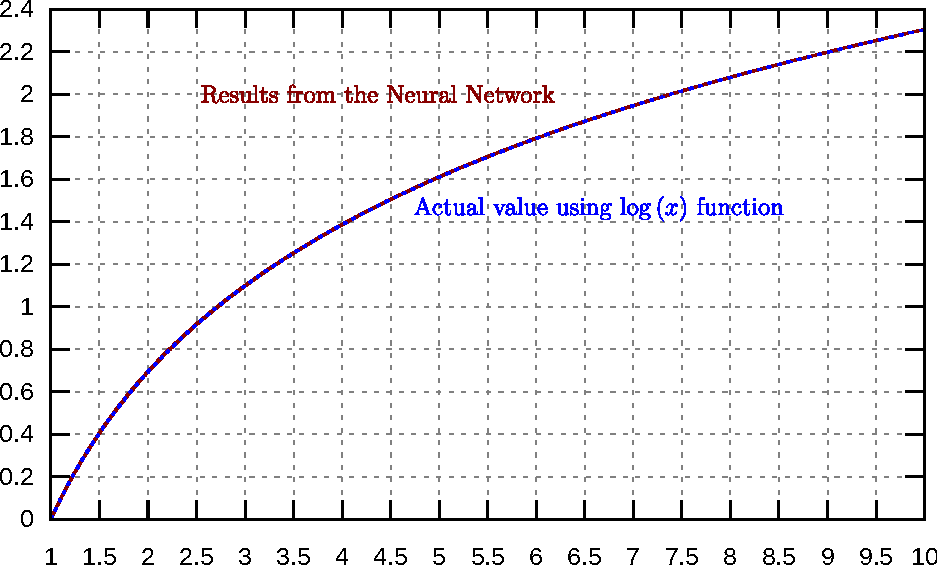
\includegraphics[width=0.8\textwidth]
        {CompareLog.pdf}
        \caption{
            Comparing solution obtained from Neural Network to the exact solution for the simple differential equation mentioned above.
        }
        \label{fig:log}
    \end{center}
\end{figure}

